\begin{frame}
    \titlepage
\end{frame}

\begin{frame}{midterm 1}
    \vspace{-.75cm}
    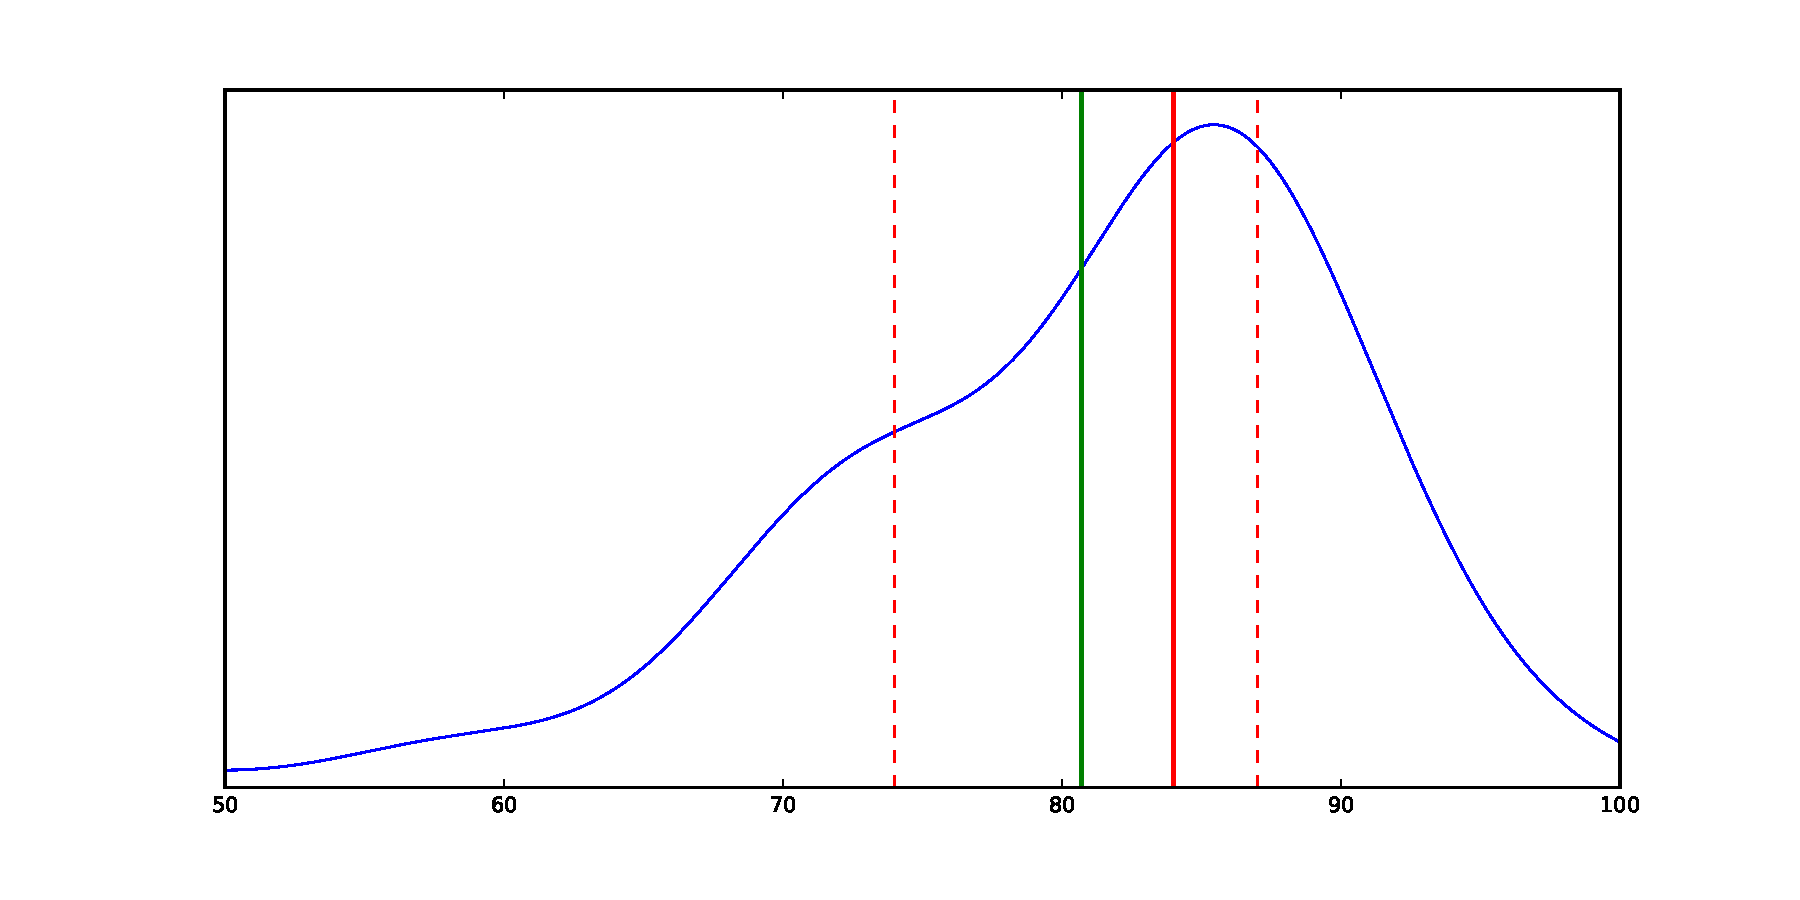
\includegraphics[width=\textwidth]{midterm1-density}
    \vspace{-.75cm}
    {\small kernel density plot; red lines: 25/50/75th perecentile; green line: mean}
\end{frame}

\begin{frame}{last time}
    \begin{itemize}
    \item stack smashing
    \item particular \myemph{exploit technique} for buffer overflows
        \begin{itemize}
        \item buffer overflow = out-of-bounds access to array
        \end{itemize}
    \item condition: buffer on the stack
    \item two steps:
        \begin{itemize}
        \item insert machine code
        \item overwrite return address to point there
        \end{itemize}
    \end{itemize}
\end{frame}

\begin{frame}<1>[label=tricky]{stack smashing: the tricky parts}
    \begin{itemize}
    \item \myemph<2>{construct machine code that works in any executable}
        \begin{itemize}
        \item same tricks as writing relocatable virus code
        \item usual idea: just execute shell (command prompt)
        \end{itemize}
    \item \myemph<3>{construct machine code that's valid input}
        \begin{itemize}
        \item machine code usually flexible enough
        \end{itemize}
    \item \myemph<4>{finding location of return address}
        \begin{itemize}
        \item fixed offset from buffer
        \end{itemize}
    \item \myemph<5>{finding location of inserted machine code}
    \end{itemize}
\end{frame}

\againframe<2>{tricky}

\begin{frame}{machine code that works anywhere}
    \begin{itemize}
        \item need \myemph{relocatable} machine code
        \item relative addressing internally
        \item absolute addressing of program
    \end{itemize}
\end{frame}

\againframe<3>{tricky}

\begin{frame}[fragile,label=valIn]{valid input?}
    \lstset{language=myasm}
    \begin{itemize}
        \item common restrictions: no {\tt 0} bytes, no newlines
        \item machine code is flexible enough, but tricky
        \item example: \lstinline|mov $0x100, %rax| has {\tt 0}s in encoding of {\tt 0x100}
\begin{lstlisting}[style=small]
        xor %eax, %eax
        mov $0x100, %al
\end{lstlisting}
    \end{itemize}
\end{frame}

\againframe<4>{tricky}

\begin{frame}[fragile,label=offsetFromRetAddr]{location of return address}
    \begin{itemize}
        \item easiest part, but \ldots
        \item depends on what compiler does
            \begin{itemize}

                \item variable number of saved registers
                \item \ldots
            \end{itemize}
        \item read assembly?
    \end{itemize}
\end{frame}

\againframe<5>{tricky}

\begin{frame}[fragile,label=stackLoc1]{stack location?}
\begin{Verbatim}[fontsize=\fontsize{9}{10}\selectfont]
$ cat stackloc.c
#include <stdio.h>
int main(void) {
    int x;
    printf("%p\n", &x);
}
$ ./stackloc.exe
0x7ffe8859d964
$ ./stackloc.exe
0x7ffd4e26ac04
$ ./stackloc.exe
0x7ffc190af0c4
\end{Verbatim}
\end{frame}

\section{mitigating stack smashing}
\begin{frame}{address space layout randomization}
    \begin{itemize}
    \item vary the location of things in memory
    \item including the stack
    \item designed to make exploiting memory errors harder
    \item will talk more about later
    \end{itemize}
\end{frame}

\begin{frame}[fragile,label=stackLoc2]{disabling ASLR}
\vspace{-.5cm}
\begin{Verbatim}[fontsize=\fontsize{9}{10}\selectfont]
$ cat stackloc.c
#include <stdio.h>
int main(void) {
    int x;
    printf("%p\n", &x);
}
$ setarch x86_64 -vRL bash
Switching on ADDR_NO_RANDOMIZE.
Switching on ADDR_COMPAT_LAYOUT.
$ ./stackloc.exe 
0x7fffffffe064
$ ./stackloc.exe 
0x7fffffffe064
$ ./stackloc.exe 
0x7fffffffe064
\end{Verbatim}
\end{frame}

\begin{frame}{finding stack location}
\begin{itemize}
\item run program in a debugger (e.g., GDB)
\item set breakpoint at relevant location 
    \begin{itemize}
    \item {\tt b functionName}
    \item {\tt b *0x12345678} (by address)
    \end{itemize}
\item output \%rsp
    \begin{itemize}
    \item {\tt p \$rsp}
    \item {\tt info registers}
    \end{itemize}
\end{itemize}
\end{frame}

\begin{frame}[fragile,label=stackLoc3]{stack location? (take 2)}
\begin{Verbatim}[fontsize=\fontsize{9}{10}\selectfont]
$ ./stackloc.exe 
0x7fffffffe064
$ gdb ./stackloc.exe
...
(gdb) break main
Breakpoint 1 at 0x4005b6
(gdb) run
Starting program: /home/cr4bd/spring2017/cs4630/slides/20170307/stackloc.exe 

Breakpoint 1, 0x00000000004005b6 in main ()
(gdb) p $rsp
$1 = (void *) 0x7fffffffdff8
(gdb) continue
0x7fffffffdfe4
[Inferior 1 (process 15441) exited normally]
(gdb) 
\end{Verbatim}
\end{frame}

\begin{frame}{Linux, initial stack}
\vspace{-1em}
\begin{tikzpicture}
\tikzset{
    stackMark/.style={draw=none,font=\it},
    envVar/.style={fill=blue!20},
    envVarP/.style={fill=violet!20},
    arg/.style={fill=green!20},
    argP/.style={fill=yellow!20},
}
\matrix[tight matrix,nodes={text width=7cm,align=center,font=\small}] (theStack){
    |[stackMark]| top of stack at {\tt 0x7ffffffff000} \\
    |[envVar]| \tt "HOME=/home/cr4bd" \\
    |[envVar]| \tt "PATH=/usr/bin:/bin" \\
    |[arg]| \tt "bar" \\
    |[arg]| \tt "foo" \\
    |[arg]| \tt "./test.exe" \\
    |[envVarP]| NULL pointer (end of list) \\
    |[envVarP]| pointer to HOME env. var. \\
    |[envVarP]| pointer to PATH env. var. \\
    |[argP]| NULL pointer (end of list) \\
    |[argP]| pointer to bar \\
    |[argP]| pointer to foo \\
    |[argP]| pointer to ./test.exe \\
    |[stackMark]| actual initial stack pointer \\
};
\node[right=1cm of theStack-1-1] (cmd) {
    {\tt ./test.exe foo bar}
};
\node[draw,envVar,right=1cm of theStack-2-1] (envVarLabel) {
    environment variables
};
\draw[thick] (theStack-2-1.north east) -- (envVarLabel.north west);
\draw[thick] (theStack-3-1.south east) -- (envVarLabel.south west);
\node[draw,arg,right=1cm of theStack-5-1] (argLabel) {
    command-line arguments
};
\draw[thick] (theStack-4-1.north east) -- (argLabel.north west);
\draw[thick] (theStack-6-1.south east) -- (argLabel.south west);
\node[draw,envVarP,right=1cm of theStack-8-1] (envVarPLabel) {
    array of pointers to env. vars.
};
\draw[thick] (theStack-7-1.north east) -- (envVarPLabel.north west);
\draw[thick] (theStack-9-1.south east) -- (envVarPLabel.south west);
\node[draw,argP,right=1cm of theStack-11-1] (argPLabel) {
    array of pointers to args (argv)
};
\draw[thick] (theStack-10-1.north east) -- (argPLabel.north west);
\draw[thick] (theStack-13-1.south east) -- (argPLabel.south west);
\end{tikzpicture}
\end{frame}

\section{debugger tutorial}

\begin{frame}{on using GDB}
    \begin{itemize}
    \item cheat sheet on website
    \end{itemize}
\end{frame}

\begin{frame}{gdb demo}
\end{frame}

\begin{frame}[fragile,label=trigSeg]{trigger segfault}
\begin{Verbatim}[fontsize=\fontsize{10}{11}\selectfont]
gdb ./a.out
...
(gdb) run <big-input.txt
Starting program: /path/to/a.out 
Program received signal SIGSEGV, Segmentation fault.
0x000000000040053b in vulnerable ()
(gdb) disass
Dump of assembler code for function vulnerable:
   0x0000000000400526 <+0>:     sub    $0x18,%rsp
   0x000000000040052a <+4>:     mov    %rsp,%rdi
   0x000000000040052d <+7>:     mov    $0x0,%eax
   0x0000000000400532 <+12>:    callq  0x400410 <gets@plt>
   0x0000000000400537 <+17>:    add    $0x18,%rsp
=> 0x000000000040053b <+21>:    retq   
End of assembler dump.
(gdb) p $rsp 
$1 = (void *) 0x7fffffffdff8
\end{Verbatim}
\end{frame}

\begin{frame}[fragile,label=trigSegStripped]{trigger segfault --- stripped}
\begin{Verbatim}[fontsize=\fontsize{10}{11}\selectfont]
gdb ./a.out
...
(gdb) run <big-input.txt
Starting program: /path/to/a.out 
Program received signal SIGSEGV, Segmentation fault.
0x000000000040053b in ?? ()
(gdb) disassemble
No function contains program counter for selected frame.
(gdb) x/i $rip
=> 0x40053b:    retq   
(gdb)
\end{Verbatim}
\end{frame}

\begin{frame}{stripping}
\begin{itemize}
\item you can remove debugging information from executables
\item Linux command: \texttt{strip}
\item GCC option \texttt{-s}
\item \texttt{disassemble} can't tell where function starts
\end{itemize}
\end{frame}

\begin{frame}[fragile,label=badDisass]{disassembly attempts}
\begin{Verbatim}[fontsize=\fontsize{10}{11}\selectfont]
gdb ./a.out
...
(gdb) run <big-input.txt
Starting program: /path/to/a.out 
Program received signal SIGSEGV, Segmentation fault.
0x000000000040053b in ?? ()
(gdb) disassemble $rip-5,$rip+1
Dump of assembler code from 0x400536 to 0x40053c:
   0x0000000000400536:  decl   -0x7d(%rax)
   0x0000000000400539:  (bad)  
   0x000000000040053a:  sbb    %al,%bl
End of assembler dump.
(gdb) disassemble $rip-4,$rip+1
Dump of assembler code from 0x400537 to 0x40053c:
   0x0000000000400537:  add    $0x18,%rsp
=> 0x000000000040053b:  retq   
End of assembler dump.
(gdb)
\end{Verbatim}
\end{frame}

\begin{frame}[fragile,label=otherAss]{other notable debugger commands}
\begin{itemize}
\item \texttt{b *0x12345} --- set breakpoint at address
    \begin{itemize}
    \item can set breakpoint on machine code on stack
    \end{itemize}
\item watchpoints --- like breakpoints but trigger on change to/read from value
    \begin{itemize}
    \item ``when is return address overwritten''
    \end{itemize}
\end{itemize}
\end{frame}

\begin{frame}{debugging demo}
\end{frame}

% FIXME: demo watchpoints

\section{stack layout skills}

% FIXME: exercise: stack layout of function with multiple choice

\section{mitigating stack smashing}

\begin{frame}<1-2>[label=stopSmashing]{stopping stack smashing?}
    \begin{itemize}
    \item how can you stop stack smashing?
    \vspace{.5cm}
    \item<2-> stop overrun --- bounds-checking
    \item<2-> \myemph<3>{stop return to attacker code}
    \item<2-> stop execution of attacker code
    \end{itemize}
\end{frame}


\begin{frame}{exploit mitigations}
    \begin{itemize}
    \item idea: turn vulnerablity to something less bad
    \item e.g. crash instead of machine code execution
    \vspace{.5cm}
    \item many of these targetted at buffer overflows
    \end{itemize}
\end{frame}

\begin{frame}{mitigation agenda}
    \begin{itemize}
        \item we will look briefly at one mitigation --- stack canaries
        \item then look at exploits that don't care about it
        \item then look at more flexible mitigations
        \item then look at more flexible exploits
    \end{itemize}
\end{frame}

\begin{frame}<1>[label=mitigationPrios]{mitigation priorities}
    \begin{itemize}
    \item \myemph<2>{effective?}\tikzmark{effective} does it actually stop the attacker?
    \item fast? how much does it hurt performance?
    \item generic? does it require a recompile? rewriting software?
    \end{itemize}

    \begin{tikzpicture}[overlay,remember picture]
        \begin{visibleenv}<2>
        \node[mycallout=effective,anchor=center,align=center] at (current page.center) {
            recurring theme: stop stack smashing, \\ but not other buffer overflows
        };
        \end{visibleenv}
    \end{tikzpicture}
\end{frame}

\subsection{stack canaries}

\againframe<3>{stopSmashing}

\begin{frame}[fragile,label=reCanary]{recall: RE}
\lstset{
    language=myasm,
    style=smaller,
    moredelim={**[is][\btHL<2|handout:0>]{~2~}{~end~}},
    moredelim={**[is][\btHL<3|handout:0>]{~3~}{~end~}},
}
\vspace{-.25cm}
\begin{lstlisting}
/* copy value from thread-local storage */
    mov ~2~%fs:0x28~end~, %rax 
/* ... on to stack, before return address */
    mov %rax, ~2~0x18(%rsp)~end~
    ...
    ...
    ...
/* copy value from stack */
    mov ~3~0x18(%rsp)~end~, %rdi
/* xor with value in thread-local storage */
    xor ~3~%fs:0x28~end~, %rdi
/* if result non-zero, do not return */
    jne call_stack_chk_fail
    add $0x28, %rsp
    ret
call_stack_chk_fail:
    call __stack_chk_fail
\end{lstlisting}
\end{frame}

\begin{frame}[fragile,label=returnToStackCanary]{stack canary}
\begin{tikzpicture}
% FIXME:
\tikzset{
    stackBox/.style={very thick},
    onStack/.style={thick},
    xscale=1.3,
}
\draw[stackBox] (0, 0) rectangle (10, -6);
\draw[thick,-Latex] (10.25,-5) -- (10.25, -1) node [midway, below, sloped] {increasing addresses};
\node[at={(5, 0.1)},anchor=south] { highest address (stack started here)};
\node[at={(5, -6.1)},anchor=north] { lowest address (stack grows here)};

\draw[onStack] (0, -.25) rectangle (10, -1.25) node[midway,align=center,font=\small] (stackAddr)
     {return address for {\tt vulnerable}: \\
     \only<1>{\fontsize{10}{11}\selectfont\tt\color{black}37 fd 40 00  00 00 00 00 (0x40fd37)}
     \only<2>{\fontsize{10}{11}\selectfont\tt\bfseries\color{red}70 fd ff ff  ff ff 00 00 (0x7fff ffff fd70)}};
\draw[onStack,fill=black!20] (0, -1.25) rectangle (10, -1.75) node[midway,align=center,font=\small] {canary: \only<1>{\tt b1 ab bd e8 31 15 df 31}\only<2>{\color{red}{\tt ?? ?? ?? ?? ?? ?? ??}}};
\draw[onStack,fill=black!20] (0, -1.75) rectangle (10, -2.25) node[midway,align=center,font=\small] {unused space (12 bytes)};
\draw[onStack,fill=blue!20] (0, -2.25) rectangle (10, -5.25) node[midway,align=center,font=\small] {buffer (100 bytes)};

\draw[onStack] (0, -5.25) rectangle (10, -6) node[midway,align=center,font=\small] {return address for {\tt scanf}};

\begin{visibleenv}<2>
\draw[-Latex,red,ultra thick] ([yshift=2.5mm]stackAddr.south east) -- ++(.25cm,0cm) |- (0.25, -5);
\node[anchor=south west,red] at (0.25, -4.75) {
    machine code for the attacker to run
};
\end{visibleenv}

\end{tikzpicture}
\end{frame}

\begin{frame}[fragile,label=stackCanaryAct]{stack canary --- action}
\lstset{
    language=myasm,
    style=small,
    moredelim={**[is][\btHL<2|handout:0>]{~2~}{~end~}},
    moredelim={**[is][\btHL<3|handout:0>]{~3~}{~end~}},
}
\begin{lstlisting}
mov %fs:0x28, %rdi //    0xb1 ab bd e8 31 15 df 31 XOR
xor %rdi, 0x112(%rsp) // 0x?? ?? ?? ?? ?? ?? ?? ??
                   // =  0x?? ?? ?? ?? ?? ?? ?? ??
jne call_stack_check_file // jump if != 0
...
call_stack_chk_fail:
  call __stack_chk_fail
  ...
__stack_chk_fail:
    /* print "*** stack smashing detected message" and exit */
\end{lstlisting}
\end{frame}

\begin{frame}{stack canary hopes}
    \begin{itemize}
    \item \myemph<2>{overwrite return address $\implies$ overwrite canary}
        \begin{itemize}
        \item<2-> buffer overrun, not some other memory error
        \end{itemize}
    \item \myemph<3>{canary is secret}
        \begin{itemize}
        \item<3-> chosen at random
        \item<3-> program doesn't output it
        \end{itemize}
    \end{itemize}
\end{frame}

\begin{frame}[fragile,label=infoDisc1]{information disclosure (1)}
\lstset{
    language=C,
    style=small
}
\begin{lstlisting}
void process() {
    char buffer[8] = "\0\0\0\0\0\0\0\0";
    char c = ' ';
    for (int i = 0; c != '\n' && i < 8; ++i) {
        c = getchar();
        buffer[i] = c;
    }
    printf("You input %s\n", buffer);
}
\end{lstlisting}
\begin{itemize}
\item input \verb|aaaaaaaa|
\item output \verb|You input aaaaaaaa|{\it (whatever was on stack)}
\end{itemize}
\end{frame}

\begin{frame}[fragile,label=infoDisc2]{information disclosure (2)}
\lstset{
    language=C,
    style=small,
}
\begin{lstlisting}
struct foo {
    char buffer[8];
    long *numbers;
};

void process(struct foo* thing) {
    ...
    scanf("%s", thing->buffer);
    ...
    printf("first number: %ld\n", thing->numbers[0]);
}
\end{lstlisting}
\begin{itemize}
\item input: {\tt aaaaaaaa}\textit{(address of canary)}
    \begin{itemize}
    \item address on stack \textit{or} where canary is read from in thread-local storage
    \end{itemize}
\end{itemize}
\end{frame}

\begin{frame}{good choices of canary}
\begin{itemize}
\item \myemph{random} --- guessing should not be practical
    \begin{itemize}
    \item not always --- sometimes static or only $2^{15}$ possible
    \end{itemize}
\item GNU libc: canary contains:
\vspace{.5cm}
    \item leading {\tt \textbackslash 0} (string terminator)
        \begin{itemize}
        \item {\tt printf \%s} won't print it
        \end{itemize}
    \item a newline
        \begin{itemize}
        \item read line functions can't input it
        \end{itemize}
    \item {\tt \textbackslash xFF}
        \begin{itemize}
        \item hard to input?
        \end{itemize}
\end{itemize}
\end{frame}

\begin{frame}{stack canaries implementation}
    \begin{itemize}
    \item ``StackGuard'' --- 1998 paper proposing strategy
    \item GCC: command-line options
        \begin{itemize}
        \item {\tt -fstack-protector} 
        \item {\tt -fstack-protector-strong} 
        \item {\tt -fstack-protector-all}
        \item one of these often default
        \item three differ in how many functions are `protected'
        \end{itemize}
    \item Microsoft C/C++ compiler: {\tt /GS}
        \begin{itemize}
        \item on by default
        \end{itemize}
    \end{itemize}
\end{frame}

\begin{frame}{stack canary overheads}
    \begin{itemize}
    \item less than 1\% runtime if added to ``risky'' functions
        \begin{itemize}
        \item functions with character arrays, etc.
        \end{itemize}
    \item large overhead if added to all functions
        \begin{itemize}
        \item StackGuard paper: 5--20\%?
        \end{itemize}
    \item similar space overheads
    \vspace{.5cm}
    \item (for typical applications)
        \begin{itemize}
        \item could be much worse: tons of `risky' function calls
        \end{itemize}
    \end{itemize}
\end{frame}

\begin{frame}{stack canaries pro/con}
    \begin{itemize}
        \item pro: no change to calling convention
        \item pro: recompile only --- no extra work
        \item con: can't protect existing executable/library files (without recompile)
        \item con: doesn't protect against many ways of exploiting buffer overflows
        \item con: vulnerable to information leak
    \end{itemize}
\end{frame}

\begin{frame}{stack canary summary}
    \begin{itemize}
    \item stack canary --- simplest of many \myemph{mitigations}
    \item key idea: detect corruption of return address
    \item assumption: if return address changed, so is adjacent token
    \item assumption: attacker can't learn true value of token
        \begin{itemize}
        \item often possible with memory bug
        \end{itemize}
    \vspace{.5cm}
    \item later: workarounds to break these assumptions
    \end{itemize}
\end{frame}

\begin{frame}{more migitations?}
    \begin{itemize}
    \item in future lectures
    \item after we talk about other ways of exploiting buffer overflows
    \end{itemize}
\end{frame}

\section{beyond stack smashing}

% FIXME: probably after simple mitigations
\begin{frame}{beyond return addresses}
     \begin{itemize}
    \item overwriting return address to point to code
        \begin{itemize}
        \item ``stack smashing''
        \end{itemize}
    \item not the only thing on the stack
        \begin{itemize}
        \item easier to overwrite something else?
        \end{itemize}
    \item some buffers are not be on the stack
        \begin{itemize}
        \item is something ``interesting'' next to them in memory?
        \end{itemize}
    \end{itemize}
\end{frame}

\againframe<2>{mitigationPrios}

\begin{frame}[fragile,label=overwriteLocal]{recall: simpler overflow}
\lstset{
    language=C,
    style=smaller,
    moredelim={**[is][\btHL<2|handout:0>]{@hi2@}{@endhi@}},
}
\begin{lstlisting}
struct QuizQuestion questions[NUM_QUESTIONS];
int giveQuiz() {
    int @hi2@score@endhi@ = 0;
    char @hi2@buffer@endhi@[100];
    for (int i = 0; i < NUM_QUESTIONS; ++i) {
        gets(buffer);
        if (checkAnswer(buffer, &questions[i])) {
            score += 1;
        }
    }
    return score;
}
\end{lstlisting}
\end{frame}

\begin{frame}[fragile,label=overwriteLocalStack]{recall: simpler overflow: stack}
\begin{tikzpicture}
\tikzset{
    stackBox/.style={very thick},
    onStack/.style={thick},
}
\draw[stackBox] (0, 0) rectangle (10, -6);
\draw[thick,-Latex] (10.25,-5) -- (10.25, -1) node [midway, below, sloped] {increasing addresses};
\node[at={(5, 0.1)},anchor=south] { highest address (stack started here)};
\node[at={(5, -6.1)},anchor=north] { lowest address (stack grows here)};

\draw[onStack] (0, -.25) rectangle (10, -1.25) node[midway,align=center,font=\small] (stackAddr)
     {return address for {\tt giveQuiz}};
\draw[onStack,fill=green!20] (0, -1.25) rectangle (10, -1.75) node[midway,align=center,font=\small] {
    score (4 bytes): \only<1>{\tt 00 00 00 00}
    \only<2>{\color{red}\tt 61 61 61 00}
};
\draw[onStack,fill=blue!20] (0, -1.75) rectangle (10, -5.25) node[midway,align=center,font=\small] {buffer (100 bytes)};

\draw[onStack] (0, -5.25) rectangle (10, -6) node[midway,align=center,font=\small] {return address for {\tt gets}};

\begin{visibleenv}<2>
\node[anchor=south west,font=\tt,red] at (0, -5.25) { aaaa\ldots };
\node[anchor=north east,font=\tt,red] at (10, -1.75) { \ldots aaaa};
\node[red] at (5, -3) {input: 103 {\tt a}'s ({\tt a} = {\tt 0x61})};
\end{visibleenv}
\end{tikzpicture}
\end{frame}

\begin{frame}{but don't you have to get lucky?}
    \begin{itemize}
        \item simple overflow seems contrived
        \item stack smashing had big advantages:
            \begin{itemize}
                \item every buffer on the stack was a problem
                \item easy to adapt exploit --- recall debugger exercise
            \end{itemize}
        \item some more exploit techniques
            \begin{itemize}
                \item not as generic as stack smashing
                \item but \myemph{collectively} close
            \end{itemize}
    \end{itemize}
\end{frame}

\begin{frame}{article on topic}
    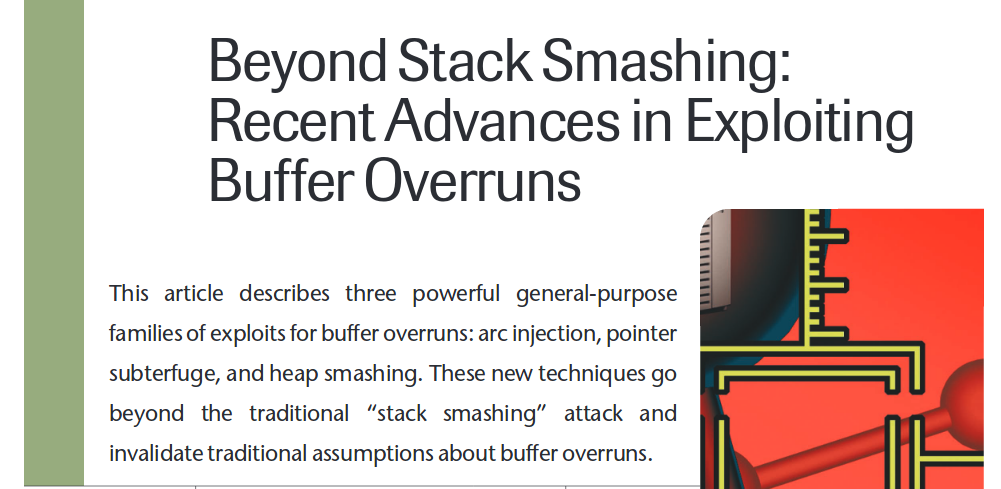
\includegraphics[width=\textwidth]{beyond-stack-smashing-title}
\end{frame}

\begin{frame}<1>[label=altExploits]{techniques from Pincus and Baker}
\begin{itemize}
\item \myemph<2>{arc injection} AKA return-oriented programming
    \begin{itemize}
    \item more detail (+ assignment) later in semester
    \end{itemize}
\item \myemph<3>{overwriting data pointers}
\item overwriting function pointers
\item overwriting pointers to function pointers
\item (on heap) overwriting {\tt malloc}'s data structures
\end{itemize}
\end{frame}

\begin{frame}{other buffer overflows?}
    \begin{itemize}
        \item old example: data on stack
    \end{itemize}
\end{frame}

\againframe<2>{altExploits}

\subsection{arc injection}

\begin{frame}[fragile,label=returnToSomewhere]{return-to-somewhere}
\begin{tikzpicture}
% FIXME:
\tikzset{
    stackBox/.style={very thick},
    onStack/.style={thick},
}
\begin{scope}[xscale=0.75]
\draw[stackBox] (0, 0) rectangle (10, -6);
\draw[thick,-Latex] (10.25,-5) -- (10.25, -1) node [midway, below, sloped] {increasing addresses};
\node[at={(5, 0.1)},anchor=south] { highest address (stack started here)};
\node[at={(5, -6.1)},anchor=north] { lowest address (stack grows here)};

\draw[onStack] (0, -.25) rectangle (10, -1.25) node[midway,align=center,font=\small] (stackAddr)
     {return address for {\tt vulnerable}: \\ address of {\tt do\_useful\_stuff}};
\draw[onStack,fill=black!20] (0, -1.25) rectangle (10, -2.25) node[midway,align=center,font=\small] {unused space (20 bytes)};
\draw[onStack,fill=blue!20] (0, -2.25) rectangle (10, -5.25) node[midway,align=center,font=\small] {buffer (100 bytes)};

\draw[onStack] (0, -5.25) rectangle (10, -6) node[midway,align=center,font=\small] {return address for {\tt scanf}};

\draw[onStack,fill=red!20,opacity=0.9] (0, -5.25) rectangle (10, -1.25) node[midway,align=center,font=\small,text=red!50!black] {unused junk};

\draw[-Latex,red,ultra thick,dashed] ([yshift=2.5mm]stackAddr.south east) -- ++(.25cm,0cm) |-
    (11, -4.25) node[align=left,right,font=\small] { {\tt do\_useful\_stuff} \\ (already in program) };

\begin{visibleenv}<2>
\fill[white,opacity=0.5, overlay] (-1,-2) rectangle (18, -8);
\end{visibleenv}
\end{scope}
\end{tikzpicture}
\begin{tikzpicture}[overlay,remember picture]
\begin{visibleenv}<2>
\node[fill=white,draw,ultra thick,align=center,anchor=center] at (current page.center) {
    code is \myemph{already in program}??? \\
    how often does this happen??? \\
    \ldots turns out ``\myemph{usually}'' --- more later in semester
};
\end{visibleenv}
\end{tikzpicture}
\end{frame}

\subsection{pointer subterfuge}

\againframe<3>{altExploits}

\begin{frame}[fragile,label=pointerSub]{pointer subterfuge}
\lstset{
    language=C,
    style=small,
    moredelim={**[is][\btHL<2|handout:0>]{~2~}{~end~}},
    morekeywords={size_t},
}
\begin{lstlisting}
void f2b(void *arg, size_t len) {
    char buffer[100];
    long val = ...; /* assume on stack */
    long *ptr = ...; /* assume on stack */
    memcpy(buff, arg, len); /* overwrite ptr? */
    ~2~*ptr = val~end~; /* arbitrary memory write! */
}
\end{lstlisting}
\imagecredit{adapted from Pincus and Baker, Figure 2}
% FIXME: stack picture
\end{frame}

\begin{frame}<1-3>[label=arbWrite]{arbitrary memory write}
    \begin{itemize}
    \item bunch of scenarios that lead to \myemph{single arbitrary memory write}
    \item how can attacker exploit this?
    \vspace{.5cm}
    \item<2-> \myemph<3>{overwrite return address directly}
    \item<2-> \myemph<4>{overwrite other function pointer?}
    \item<2-> overwrite existing machine code (insert jump?)
    \item<2-> overwrite another data pointer --- copy more?
    \end{itemize}
\end{frame}

\begin{frame}[fragile,label=skipCanary]{skipping the canary}
\begin{tikzpicture}
% FIXME:
\tikzset{
    stackBox/.style={very thick},
    onStack/.style={thick},
}
\begin{scope}[xscale=1.2]
\draw[stackBox] (0, 0) rectangle (10, -6);
\draw[thick,-Latex] (10.25,-5) -- (10.25, -1) node [midway, below, sloped] {increasing addresses};
\node[at={(5, 0.1)},anchor=south] { highest address (stack started here)};
\node[at={(5, -6.1)},anchor=north] { lowest address (stack grows here)};

\draw[onStack] (0, -.25) rectangle (10, -1.25) node[midway,align=center,font=\small] (stackAddr)
     {return address for {\tt f2b} };
\draw[onStack,fill=red!20] (0, -1.25) rectangle (10, -2.25) node[midway,align=center,font=\small] (canaryAddr)
     {stack canary};
\draw[onStack,fill=green!20] (0, -2.25) rectangle (10, -2.75) node[midway,align=center,font=\small] (ptr) {ptr (8 bytes)};
\draw[onStack,fill=green!20] (0, -2.75) rectangle (10, -3.25) node[midway,align=center,font=\small] (val) {val (8 bytes)};
\draw[onStack,fill=blue!20] (0, -3.25) rectangle (10, -5.25) node[midway,align=center,font=\small] {buffer (100 bytes)};

\draw[onStack] (0, -5.25) rectangle (10, -6) node[midway,align=center,font=\small] {return address for {\tt scanf}};

\begin{visibleenv}<2->
\draw[-Latex,orange,ultra thick] ([xshift=1cm]ptr.east) -- ++(2cm,0cm) |- (stackAddr.east);
\draw[-Latex,orange,ultra thick,dashed] ([xshift=1cm]val.east) -- ++(2cm,0cm) |- (0.25, -5);
\end{visibleenv}

\begin{visibleenv}<3>
\draw[-Latex,red,ultra thick] ([yshift=2.5mm]stackAddr.south east) -- ++(.25cm,0cm) |- (0.25, -5);
\node[anchor=south west,red] at (0.25, -4.75) {
    machine code for the attacker to run
};
\end{visibleenv}
\end{scope}

\end{tikzpicture}
\end{frame}

\begin{frame}{fragility}
\begin{itemize}
\item problem: need to know exact address of return address
\item discussed how stack location varies --- this is tricky/unreliable
\end{itemize}
\end{frame}
